\documentclass[11pt,a4paper,twoside]{book}
\usepackage[utf8]{inputenc}
\usepackage[spanish]{babel}
\usepackage{amsmath}
\usepackage{graphicx}
\usepackage{amsfonts}
\usepackage{amssymb}
\usepackage[left=2cm,right=2cm,top=2cm,bottom=2cm]{geometry}
\usepackage{float}
\author{Víctor de Tejada Molera}
\begin{document}
    \chapter{Desarrollo de la aplicación del test subjetivo.}
        En este capítulo se explican las herramientas y lenguajes utilizados para la creación de la aplicación de escritorio con la que se realizan posteriormente los test subjetivos de audio necesarios para el proyecto. Así mismo, se explica el algoritmo utilizado y las diferentes versiones utilizadas para la creación de la interfaz de usuario.
        
        \section{Lenguajes y programas utilizados}
            Para el desarrollo de la aplicación, se ha optado por utilizar el lenguaje de programación Python3. Este lenguaje tiene la ventaja de que incluye numerosas librerías que permiten trabajar con interfaces gráficas con las que los participantes de los test puedan interactuar de forma sencilla. Para nuestro caso particular, se ha optado por utilizar la librería del entorno gráfico GTK (la librería se llama \textit{PyGObject}\footnote{https://pygobject.readthedocs.io/en/latest/}) que es una de las más utilizadas en entornos Linux, aunque también puede utilizarse en entornos de Windows o Mac.
            
            Para el diseño de la interfaz, se podría haber codificado diréctamente en lenguaje python. No obstante, se ha utilizado el programa Glade que permite utilizar un entorno gráfico para la creación de todos los elementos de la interfaz. Con dicho programa se obtiene un fichero XML con extensión ``.glade'' que es el que el \textit{script} de Python lee y con el que se genera la interfaz que el usuario utiliza. En la figura \ref{fig:gladeInic} se puede observar la pantalla de inicio de dicho programa. 
            
            \begin{figure}
                \begin{center}
                    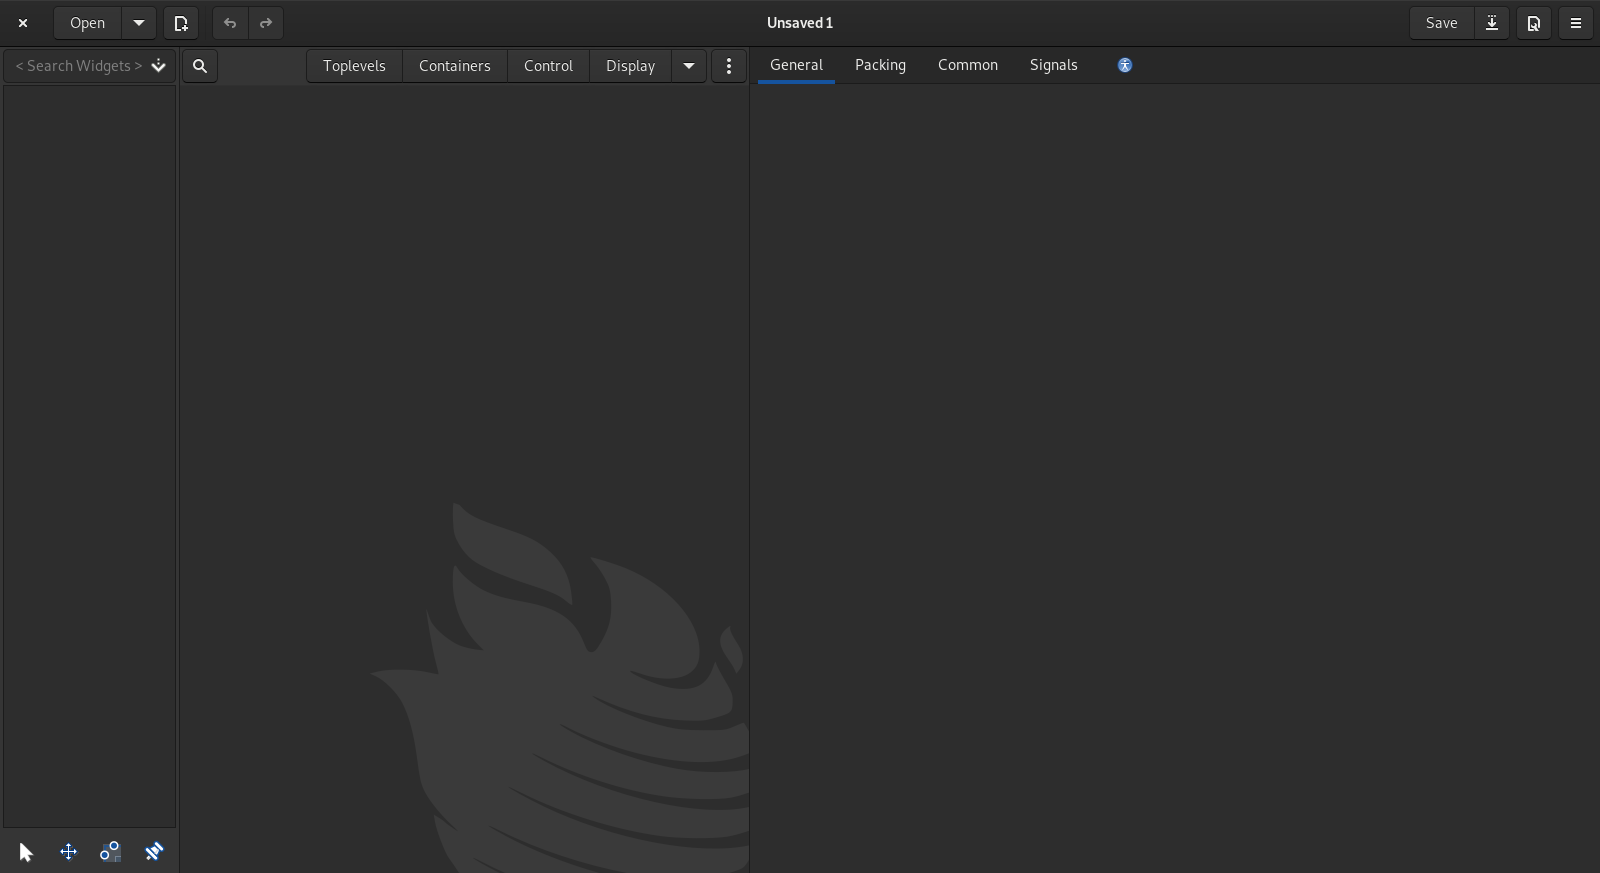
\includegraphics[scale=.2]{../imagenes/gladeInicio.png}
                    \caption{Ventana de inicio del programa \textit{Glade}.}
                    \label{fig:gladeInic}
                \end{center}
            \end{figure}
            
           \newpage

           Para la codificación de los scripts de Python se ha utilizado el programa ``\textit{Gnome Builder}''; un entorno de aplicaciones que incluye todas las herramientas para depurar, compilar y ejecutar los scripts dentro del mismo espacio. Al igual que con \textit{Glade}, el programa es gratuito de código abierto. En la figura \ref{fig:builderIni} se encuentra una captura de la interfaz del programa.
           
            \begin{figure}[H]
                \begin{center}
                    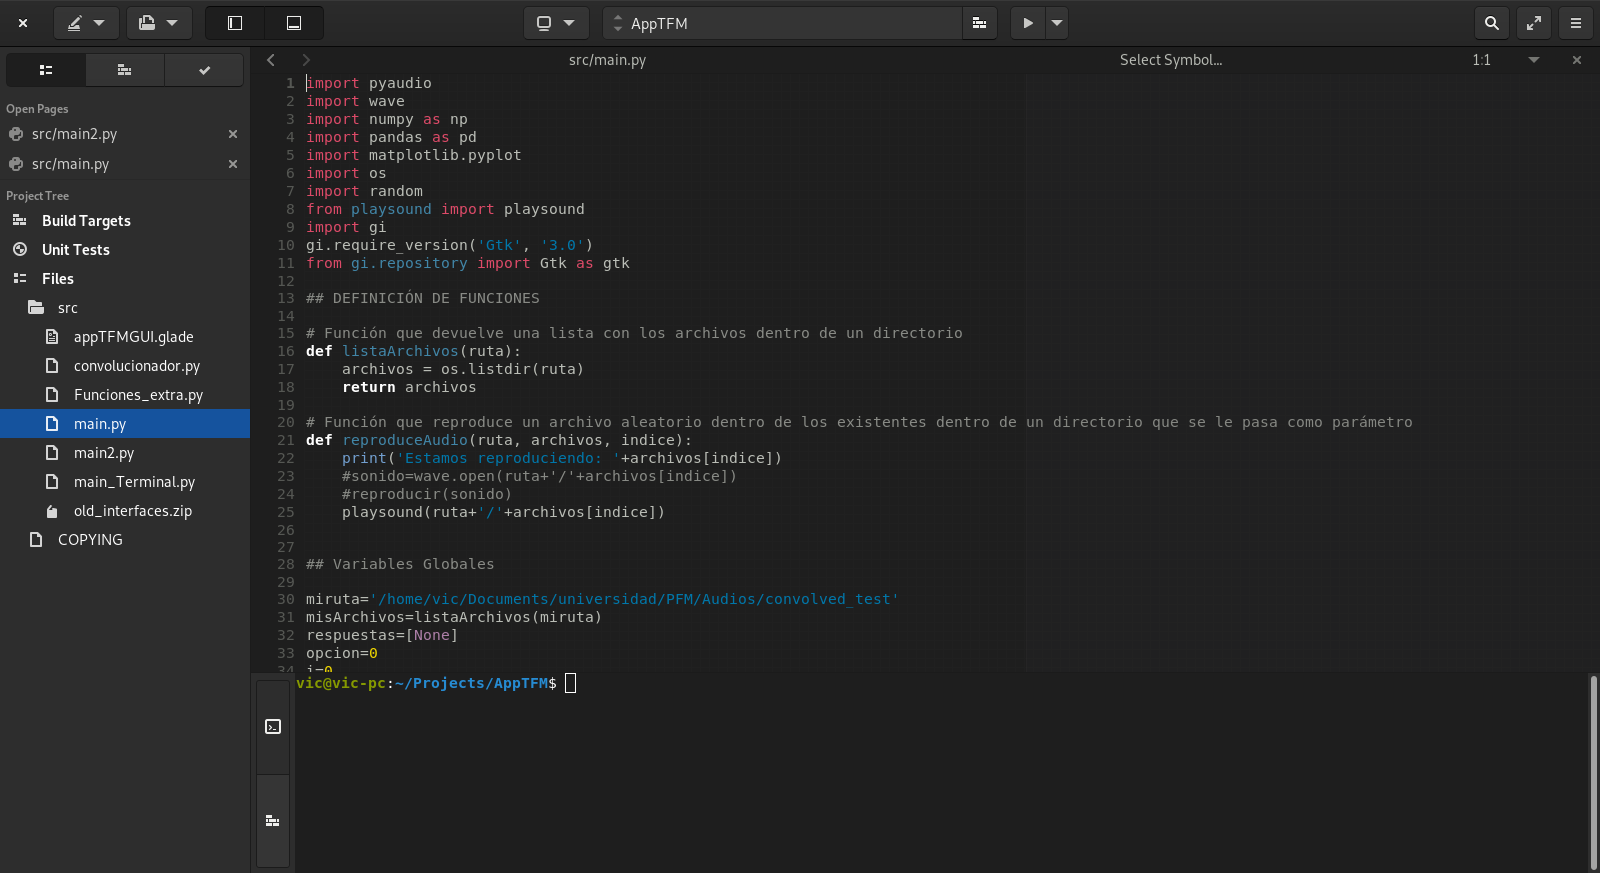
\includegraphics[scale=.2]{../imagenes/builderIni.png}
                    \caption{Captura del programa \textit{Gnome Builder}.}
                    \label{fig:builderIni}
                \end{center}
            \end{figure}
            
        \section{Características de la interfaz de usuario}
            Como se ha comentado en el apartado anterior, la interfaz de usuario se ha diseñado utilizando el programa ``\textit{Glade}''. Desde un principio, se ha querido diseñar una interfaz que sea lo más simple posible, no sólo por facilidad para realizarla, sino para que las personas participantes puedan centrarse exclusivamente en los aspectos del test y hacer que su uso no suponga ninguna dificultad.  
            
            En una primera instancia se decidió generar una interfaz en la que los elementos principales fueran dos botones con los que el usuario pudiera escoger cuál de los audios quería reproducir. Las respuestas se recogerían en dos casillas, o \textit{toggles}. También se incluyó un botón en la parte inferior para enviar cada una de las respuestas. En la parte superior se incluye un texto que indica el número de pregunta por la que va el test. Todos estos elementos se pueden observar en la figura \ref{fig:uiIni}.
            
            \begin{figure}[H]
                \begin{center}
                    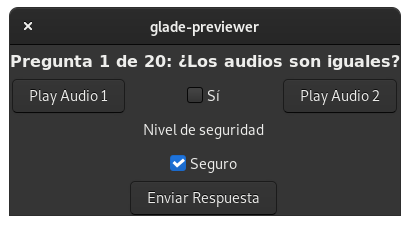
\includegraphics[scale=.6]{../imagenes/uiIni.png}
                    \caption{Versión inicial de la interfaz de usuario.}
                    \label{fig:uiIni}
                \end{center}
            \end{figure}
            
            Esta configuración es la que se utiliza en el test previo. Al finalizar dicho test, se les pidió a los participantes que propongan diferentes mejoras para perfeccionar la interfaz de usuario. Entre ellas, las más habituales consistieron en la sustitución de los \textit{toggles} por elementos más grandes al estilo de \textit{switches} o interruptores y la actualización de la posición de dichos elementos a su estado inicial entre cada una de las preguntas.
            Atendiendo a estas propuestas, se modifica la interfaz con el resultado que se muestra en la figura \ref{fig:uiFin}.
            
            \begin{figure}
                \begin{center}
                    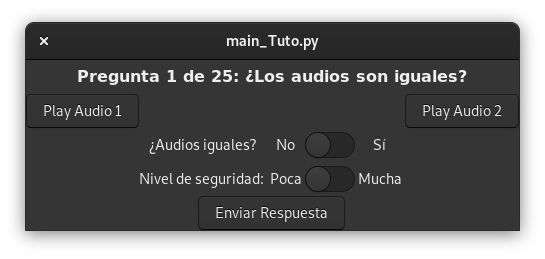
\includegraphics[scale=.6]{../imagenes/interFin.png}
                    \caption{Versión inicial de la interfaz de usuario.}
                    \label{fig:uiFin}
                \end{center}
            \end{figure}
            
        \section{Codificación del script en Python}            
            El procedimiento seguido para la codificación de la aplicación ha sido gradual. En primer lugar se han diseñado diferentes métodos y funciones que se apliquen diréctamente desde la consola. De esta forma, se comprueba que el algoritmo funciona correctamente y que se extraen los resultados en el formato deseado.
            
            Una vez, se ha comprobado que este \textit{script} funciona, se modifica el mismo haciendo que las diferentes funciones sean llamadas por los diferentes elementos de la interfaz de usuario ya creada y que se referencian dentro del código de Python.
            
            Durante todo el proceso, se realizaron consultas a la documentación de la API de Python para GTK\footnote{https://python-gtk-3-tutorial.readthedocs.io/en/latest/} y de las diferentes librerías necesarias para el desarrollo de la aplicación. Varios ejemplos de estas librerías son:
            \begin{itemize}
                \item \textbf{numpy}\footnote{https://numpy.org/}: para el trabajo con matrices al estilo de programas como \textit{Matlab}.
                \item \textbf{pandas}\footnote{https://pandas.pydata.org/}: para la edición y creación de estructuras de datos.
                \item \textbf{os}\footnote{https://docs.python.org/3/library/os.html}: para la navegación dentro de sistemas de ficheros del sistema operativo.
                \item \textbf{gi}\footnote{https://pygobject.readthedocs.io/en/latest/guide/api/api.html}: para el manejo de los elementos gráficos y la gestión de sus señales.
            \end{itemize}
            
            Por último durante el periodo de tiempo entre los dos tests subjetivos de audio se añadió la funcionalidad que permitía reproducir los dos audios pulsando las teclas ``1'' y ``2'' del teclado respectivamente sin necesidad de utilizar el ratón. Esta funcionalidad se incorporó como sugerencia por parte de varias de las personas participantes que comunicaron las dificultades de escuchar los audios con los ojos cerrados (decisión personal) al tener que pinchar los botones con el ratón del ordenador.
            
            \subsection{Estructura del código}
                El código de Python se encuentra dividido en diferentes partes:
                En primer lugar, la zona donde se importan las diferentes librerías para el correcto funcionamiento del script. Aquí se incluyen las que permiten reproducir los diferentes audios, manejar información, navegar por el sistema de archivos del ordenador, la interfaz gráfica, etc.
                
                A continuación, se encuentra una zona donde se definen diferentes funciones que serán usadas repetidamente a lo largo del \textit{script}. 
                
                Después, se definen algunas variables globales necesarias y da comienzo la clase \textit{Main} de la aplicación. En ella, se inicializan las referencias a los diferentes elementos de la interfaz gráfica con las que los usuarios interactúan y se establecen qué funciones se llaman en función de las señales que manejan. Estas funciones se definen en último lugar a continuación de dichas inicializaciones. En el anexo X se puede leer el código en su totalidad.
               
        
\bibliography{biblio.bib}
\bibliographystyle{ieeetr}
\end{document}